\documentclass{article}
\usepackage{graphicx}
\usepackage[margin=1.5cm]{geometry}
\usepackage{amsmath}

\begin{document}

\title{Warm Up: Centripetal Acceleration, Circular Motion, and Applied Forces}
\author{Prof. Jordan C. Hanson}

\maketitle

\section{Memory Bank}

\begin{itemize}
\item $s = r\theta$ ... Let $s$ be the \textit{arc length} around a curve, with $r$ being the radius of curvature, and $\theta$ being angle between the initial and final position vectors.
\item $a_{\rm C} = v^2/r$ ... The centripetal acceleration given the speed $v$ around a circular path $r$.
\end{itemize}

\begin{figure}
\centering
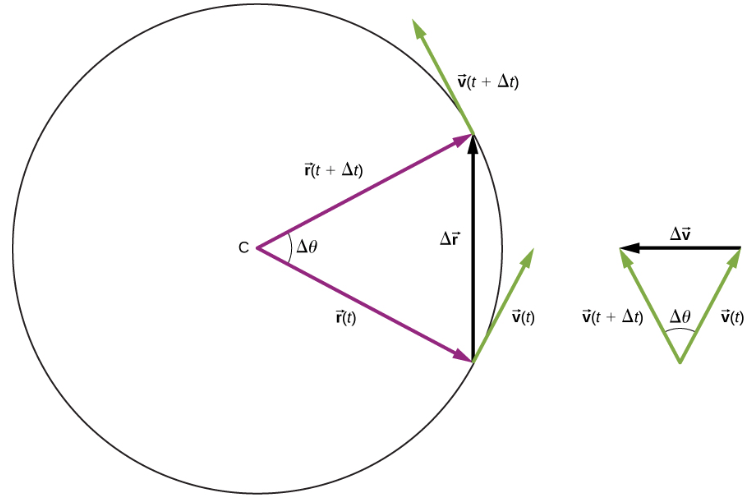
\includegraphics[width=0.345\textwidth]{figures/circle.png} \hspace{1cm}
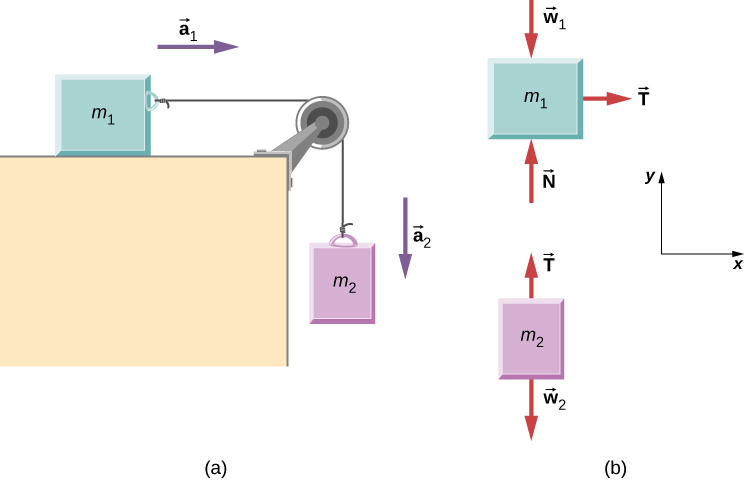
\includegraphics[width=0.45\textwidth]{figures/blocks.jpg}
\caption{\label{fig:circle} (Left) The origin of centripetal acceleration.  (Right) A pulley system with two masses.}
\end{figure}

\section{Uniform Circular Motion: Curved Coordinates}

\begin{enumerate}
\item Suppose a circular path as a radius of $10$ m.  If we travel 10 degrees around the circle, how far have we walked? \\ \vspace{0.5cm}
\item If we walk $200$ meters along a circular path, and later determine that our direction changed by 90 degrees (say, from North to West), what was the radius of curvature? \\ \vspace{0.5cm} 
\item In Fig. \ref{fig:circle} (left), a system moves in a circle with speed $v$.  The velocity changes direction by an angle $\Delta\theta$, as does the position.  It may be shown that this leads to \textit{centripetal acceleration}, $a_{\rm C}$.  (a) If a system is moving at 4 m/s around a curve with radius 0.25 m, what is $a_{\rm C}$? (b) What is $a_{\rm C}$ if $r = 1$ m?
\end{enumerate}

\section{Applied Forces, II}

\begin{enumerate}
\item Assuming there is no friction on $m_1$ in Fig. \ref{fig:circle} (right), derive an expression for the acceleration of $m_2$.  Start with the free-body diagram of each block, and assume both blocks are accelerating.
\end{enumerate}

\end{document}
